\chapter{Data Reduction and Analysis}
	\label{cha:Data}
% In Section \ref{sec:}, we lay out the the Southern Sample.


\section{VIMOS}
	\label{sec:VIMOS}
	\subsection{The VIsable Multi-Object Spectrograph (VIMOS)}
	% Details of VIMOS instrument
		%
		The sample was observed with the VIsable Multi-Object Spectrograph (VIMOS), mounted on UT3 on the VLT in Paranal \citep{LeFevre2003}, using the new (at the time) HR Blue grism. All observations were taken with a spacial resolution of 0.67". Each object was imaged with a total integration time of $\sim 100$ mins equally spread over three observing blocks. Each block contained all of the necessary calibration images (3 flat fields and 1 He and Ne arc lamp image for wavelength calibration), as well as two science pointings. In addition, VIMOS provides 5 bias images per night. Flux calibrations was done using public Standards provided by ESO of Feige 110.

		%
		VIMOS has several well known, though not well understood technical issues. These include several low transmission (bad) fibers, strong flexure and large differences in sensitivity across its 4 separate detectors, known as quadrants. These are addressed by a specialist data reduction pipeline as described in Section \ref{subsec:reduct}. 

	\subsection{Observations with VIMOS}
	% Details of observations: when, how
	\subsection{Data Reduction of VIMOS Data}
		%
		The data reduction pipeline was produced using \textsc{Py3D}, a suite of programs based on those developed for Califa DR1 \citep{Sanchez2011, Husemann2013} and later updated for VIMOS by \citet{Husemann2014}. This pipeline accounts for many of the known issues with VIMOS such as bad fibers and strong flexure. A brief outline is the additional steps to accounts for these is given below, while detailed descriptions can be found in \citet{Sanchez2011} for the standard reduction steps (bias subtraction, flat-fielding and wavelength and flux calibrations) and \citep{Husemann2014} for the VIMOS specific modifications. 
		\begin{itemize}
		\item The known bad pixels and flexure offsets are included when completing the wavelength calibration. In testing, this was found to be robust except for the blue end of the spectrum ($\lambda < 4300 \AA$) when using the blue HR grism \citep{Husemann2014}. Indeed, we found that the spectrum below the 4000\AA break was not robust and was therefore discarded.
		\item Flexure also gives an offset to flat-fielding and while this known to be only up to $\pm0.5$pixels, this is also taken into account.
		\item The dense packing of the fibers onto the CCD means that cross-talk is occurs and is extracted using \citep{Horne1986}. 
		\end{itemize}
		All of the above steps are detailed in Section 2.3 in \citet{Husemann2014}.

		%After inspecting the reduced data cubes, it was noted that most of the outer fibres had no (or very low) transmission. Given the observations were all centally located on the field of view, the outer 2 rows of fibres on each edge were able to be discarded to leave a final cube of the central 36 x 36 fibres or a field of view of 24.1 x 24.1 arcsecs. 

		%
		Following on from this, it was noted that the cubes where still not fully corrected. A fringe-like pattern was still observable in the spectral direction and quadrants were not calibrated to each other. These were improved by implementing a \textsc{python} version of the ad-hoc corrections given in \citet{Lagerholm2012}. This involves re-normalizing the quadrants by minimizing the difference of the integrated spectra in neighboring fibers (Q2 was held constant) followed by the removal of a fringe-like pattern, by dividing out a smoothed median spectrum from the eight surrounding fibers of any given fiber, over a scale of 150 pixels. These steps mean that the data-cubes will not be flux-calibrated, however the effect is multiplicative and thus will not effect equivalent width measurements.  

		%
		The variance spectra is propagated throughout the data reduction pipeline to be used a noise input in the analysis (\S \ref{sec:analysis})

	\subsection{Data Quality}
\section{MUSE}
	\label{sec:MUSE}
	\subsection{The Multi-Unit Spectroscopic Explorer (MUSE)}
		%
		Four of the sample (IC1459, IC1531, NGC1316 and NGC1399) where found to be in the archive for the Multi-Unit Spectroscopic Explorer (MUSE). NGC1316 and NGC1399 where both observed as mosaics, while IC1459 and IC4296 where observed in single pointing. All were observed in the wide-field mode without adaptive optics. The phase 3 (pre-reduced) data products from ESO were used. 

	\subsection{MUSE Archival Observations}


	\subsection{Reducing MUSE Data}
		%
		As stated in section \ref{subsec:MUSE}, we used the supplied, reduced data product, however it was noted that the sky for both IC1459 and IC426 had been over subtracted leading to large apparent absorption features (often with negative fluxes). To remove this over-subtraction, our own pseudo-sky subtraction routine was developed. The median spectrum was taken from four 20x20 spaxel boxes taken from each corner of the observation. After checking that no stellar continuum could be fitted to the spectrum (i.e. there was very little light from the galaxy contaminating our pseudo-sky spectrum), this spectrum was subtracted from each spaxel in the cube. The data-cubes were then trimmed to the central 30"x30" (150x150 spaxels).


\section{Data Analysis}
	\label{sec:analysis}
	%
	From this point on, the two datasets are treated almost identically. The only difference (other than the different spectral range and resolutions) is that the MUSE datacubes were binned to a higher signal to noise ratio (S/N).



	%
	The entire pipeline summed up is as follows:
	\begin{enumerate}
		\item Spatial binning using Voronoi binning
		\item Find relevant stellar templates by fitting the entire galaxy spectra with all the templates from the Miles library
		\item Estimate redshifts and global line-of-sight velocity dispersion with MCMC routine 
		\item Find bestfitting LOSVD for each individual bin
		\item Use bootstrapping method to estimate uncertainties LOSVD measurements. 
	\end{enumerate}





	\subsection{Spatial Binning}
		%
		Given that galaxy (the signal) is brightest at the center and fades away radially, while the noise, which is assumed to be Poisson dominated scales as the square root of the signal, the S/N will be highest at the center, decreasing with increasing radius. In the out regions of a galaxy, it becomes too low for to make meaningful fits to the spectra. Because of this we spatial bin to a set S/N (increasing a bins size until it reaches the require S/N). We do this using a Voronoi Binning routine\footnote{http://www-astro.physics.ox.ac.uk/~mxc/software/} by \citet{Cappellari2003}. This  which is fast becoming an 'industry standard' method for adaptive 2D binning. To do this, we defined 'signal' and 'noise' as the median value of the spectrum and noise spectrum respectively for each spaxel, and required a target S/N of 30 for all VIMOS datacubes, 50 for IC 1459 and IC 4296 MUSE datacubes and 100 for NGC 1316 and NGC 1399 datacubes. The MUSE datacubes had differing S/N due to the sky subtractions that were applied. These were successful in removing artifacts from the spectra of IC 1459 and IC 4296 which allowed us to retain a higher level of spatial information (by binning to a lower S/N) for these two galaxy. Unfortunate they were not appropriate for the observations of NGC 1316 and NGC 1399 due to the angular size of these objects and the tessellated nature of the their observations (see section \ref{sec:skysubtractions}). Figure \ref{fig:egSNR} shows an example of the S/N of the bins. In it, concentric ringed structures can be clearly seen around the center of the galaxy as bins with a S/N just below to target are increased in size by a single spaxel meaning they have a final S/N well over the target.

		%
		% Need to remove bin numbers, galaxy name and redshift and second axis from plot.
		\begin{figure}
			\centering
			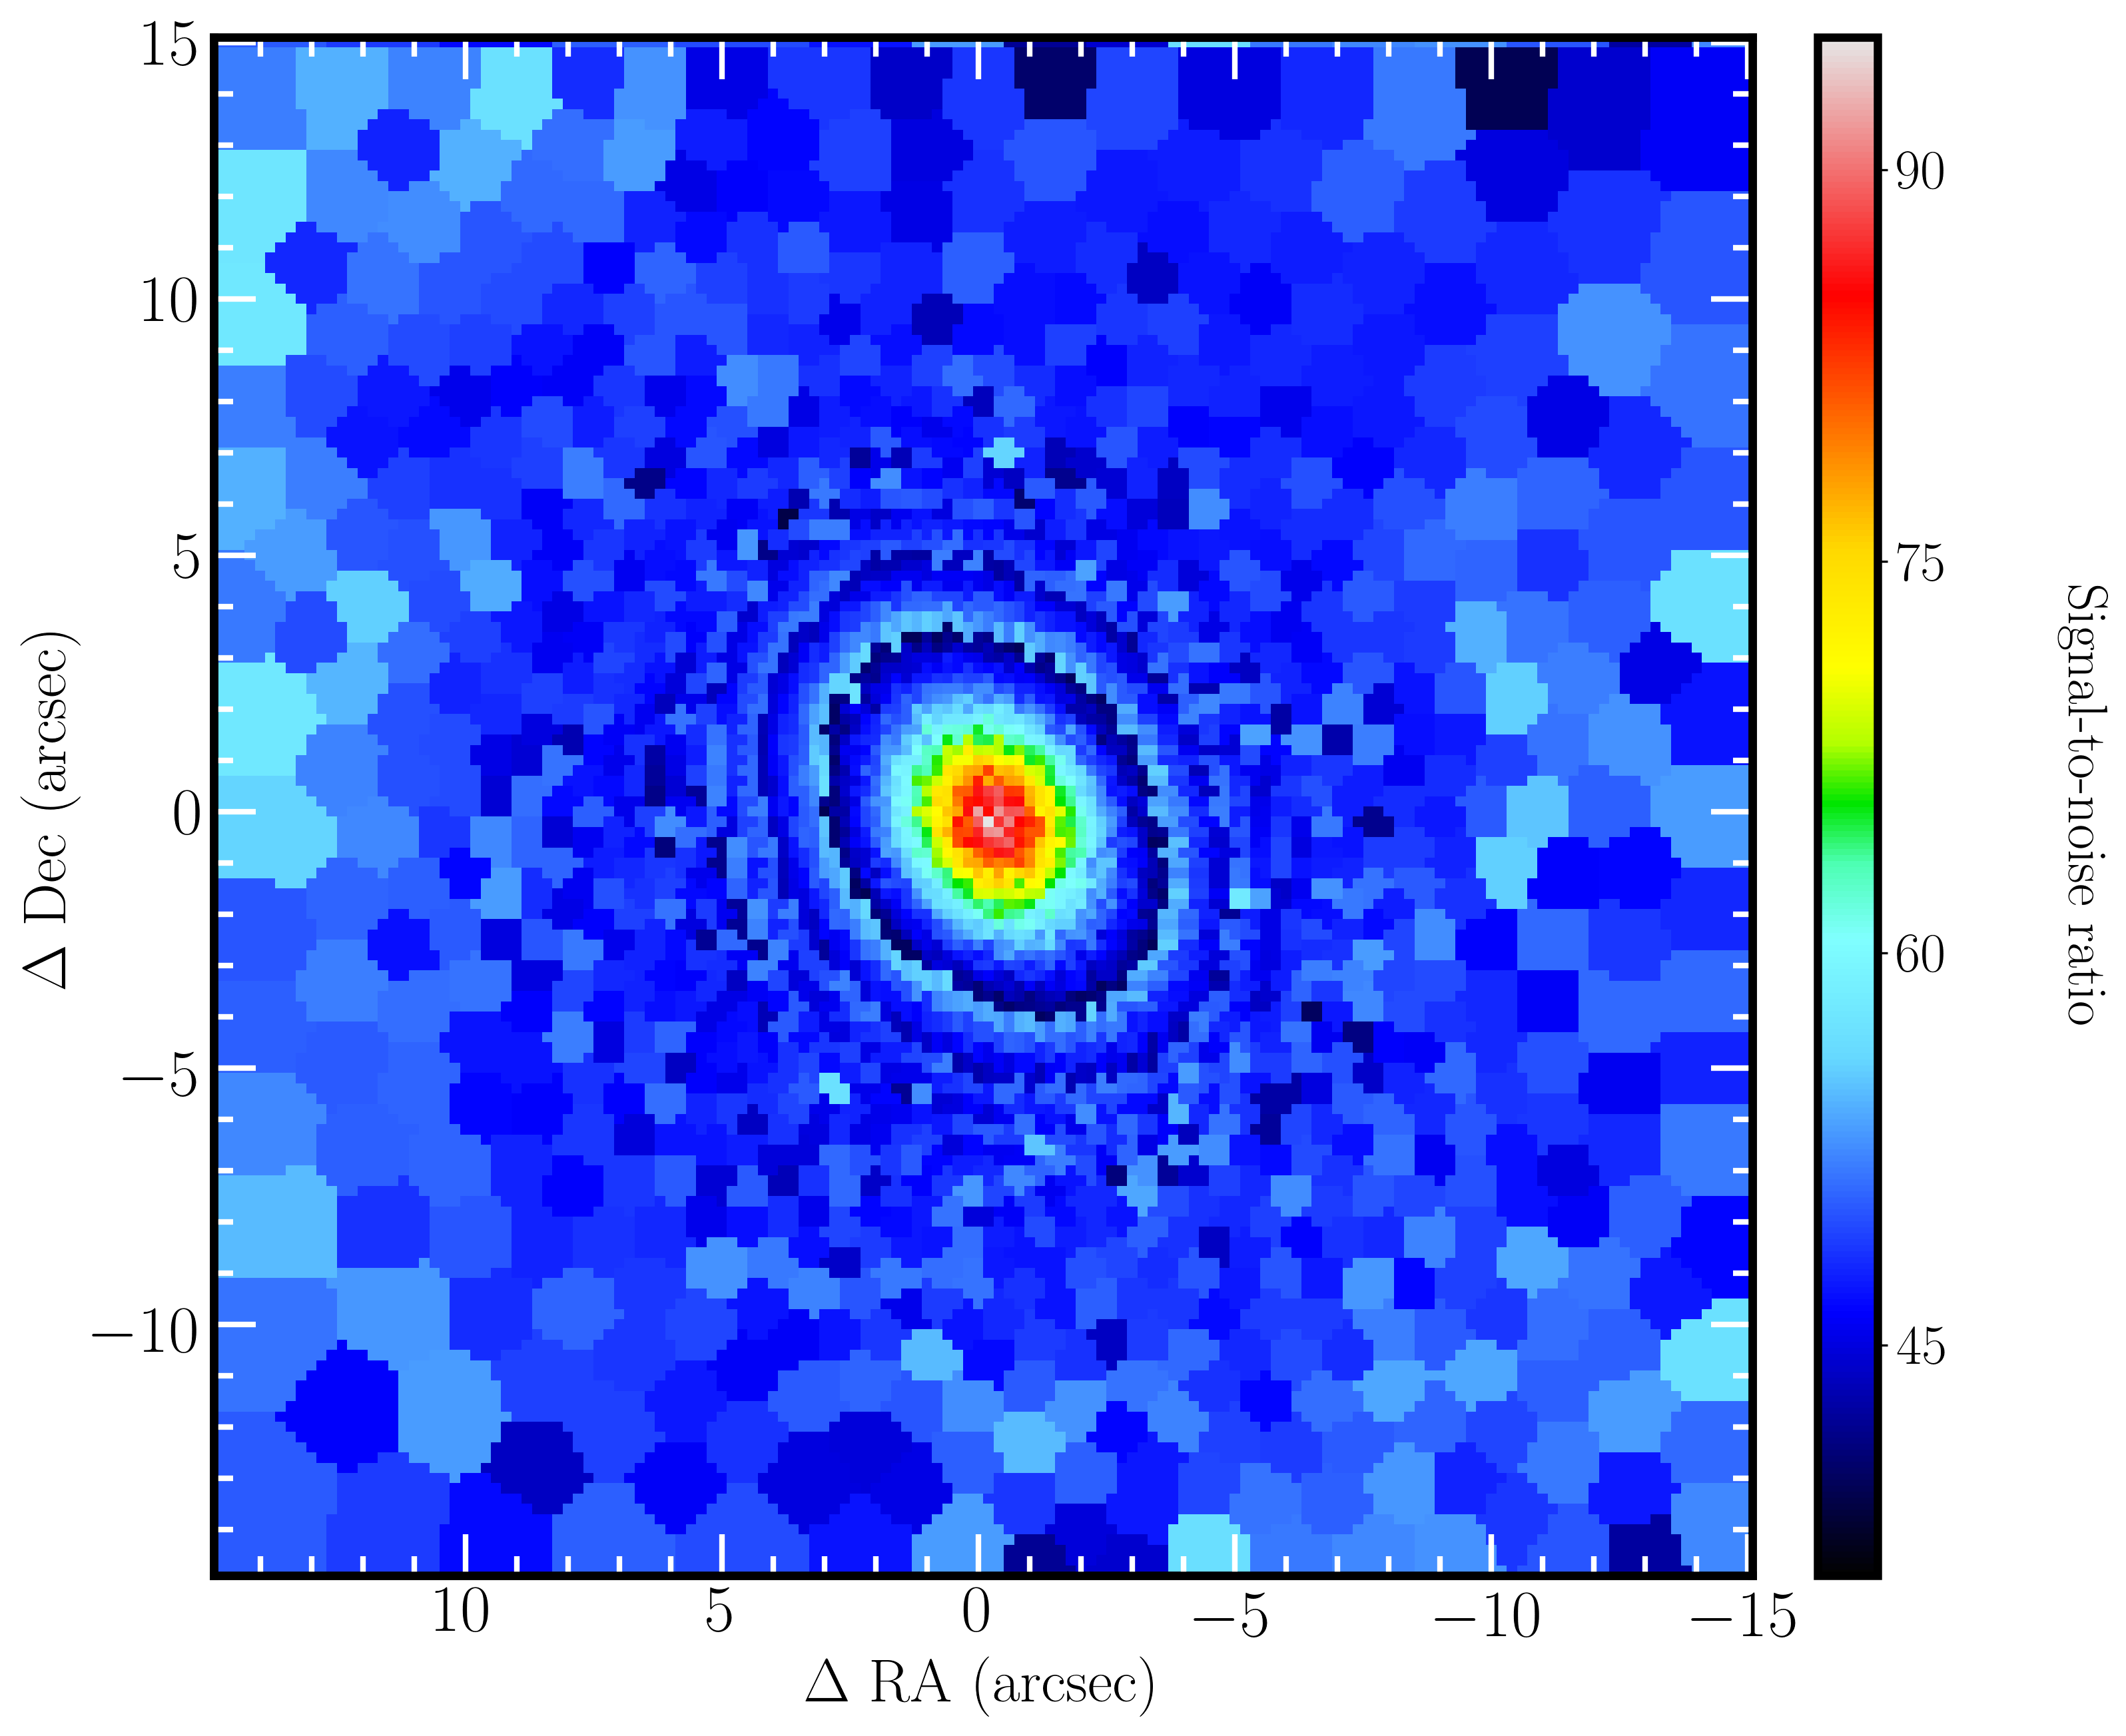
\includegraphics[width=.6\textwidth]{chapter2/egSNR.png}
			\caption[Example S/N map]{The figure shows an example S/N map (color scale) for the MUSE observation of IC 1459. The flux contours are shown in black.}
			\label{fig:MassRe}
		\end{figure}

		%
		Our analysis makes use of the penalized-fitting routine \textsc{ppxf}\footnote{\textsc{IDL} and \textsc{Python} routines for \textsc{ppxf} can be found at http://www-astro.physics.ox.ac.uk/~mxc/software/} by \citet{Cappellari2004, Cappellari2016a}. This routine finds the bestfitting spectra by building galactic spectra from combined stellar templates and convolving them with a Gaussian line-of-sight velocity distribution (LOSVD, we did not allow any deviations from a Gaussian profile for the stellar fits). Additive and multiplicative corrections to the continuum level can also be included in the fit using Lagrange polynomials. Regions (800 km s$^-1$ wide) around possible emission lines were masked. Emission lines included were: [OII]3726 , [OII]3729, H$_\delta$, H$_\gamma$, H$_\beta$, [OIII]4959, [OIII]5007, [NI]5199, [NI]5202, [OI]6300, [OI]6364, [NII]6548, [NII]6583, H$_\alpha$, [SII]6716 and [SII]6731. A telluric line at 5199 \AA, seen in some of the VIMOS spectra, was also masked, though the exact location of this depended on the initial redshift 'guess' since the spectrum is moved to the rest frame of the galaxy. For this analysis, we also allowed an additive continuum correction using a fourth order Lagrange polynomial.

		%
		In order to improve the speed of our analysis, we first collapse the datacube spatially to give global spectra for the galaxy. Obviously this means that the contribution from each spaxel is weight by its luminosity. Then the entire Miles stellar library \citep{} is used as templates for \textsc{ppxf} to fit. For our 14 datacubes (10 VIMOS and 4 MUSE), this step fits an average of \_\_\_\_\_\_ out of 985 templates with a weighting of zero. When a template for a particular datacube is given a zero weighting at this step it is not used for future analysis of that datacube. This drastically improves the runtime of \textsc{ppxf} without effecting the quality of the fit. For this fit the redshift from Simbad is used to move the spectra to the rest frame such that an initial guess of the velocity within that frame is 0 km s$^{-1}$. We use a initial guess of the velocity dispersion of 200 km s$^{-1}$ since ETGs have dispersions of around this value and higher. 

		%
		Next we run a very simply Markov chain Monte Carlo (MCMC) routine to find more optimum initial guesses for velocity and velocity dispersion. The initial run is set up in the same way as the previous step (though only using the templates with non-zero weightings). After each run, the fitted velocity and velocity dispersion were used to iteratively improve the initial guess for the next run. After the first three reps, the velocity was used to calculate the redshift of the galaxy: these are the redshift values quoted in \ref{tab:sample}. After this 100 reps were run with the mean velocity (in the de-redshifted frame) and velocity dispersion were recorded and used as the initial guesses for all fits in that datacube. 

		%
		Beyond this point, each bin is analyzed independently. Each one is processed through \textsc{ppxf} using only the Miles templates with non-zero weighting from above, using the redshift, additional velocity and dispersion estimates from the last step.


	\subsection{Stellar Kinematics}
		%
		Following this the cubes were analyzed using the \textsc{pPXF} package \citep{Cappellari2004} to find a best fit spectrum by stacking the Miles empirical stellar spectra \citep{Sanchez-Blazquez2006} convolved with a line-of-sight velocity distribution (LOSVD) given by a Gaussian-like distribution, allowed to vary up to the 4th Gauss-Hermite moment (i.e. the LOSVD could be characterized by 4 parameters: recessional velocity, $v$; line-of-sight velocity dispersion, $\sigma$ and the 3rd and 4th Gauss-Hermite moments, $h_3$ and $h_4$). To allow accurate estimation of the uncertainties in these values, a simple Monty Carlo (MC) method with 1000 repeats was used. In each iteration, random noise, with an amplitude comparable to the noise propagated through the data reduction pipeline, was added to the original bestfit spectrum.



	 \subsection{Emission-line Kinematics}
	 	%
	 	In order to combat template mismatch in the fitting of emission lines, we follow the recipe set out in \citet{Sarzi2005}. This is a three step process:
		\begin{enumerate}
			\item the region encompassing $\pm 300 \mathrm{km s^{-1}}$ around each emission line's rest frame wavelength is masked, and the stellar spectrum is fitted.
			\item The kinematics of the stellar spectrum is then fixed to the kinematics found in Step 1. The region around the [OIII] line is unmasked and fitted. In VIMOS data, the line is given just 2 free kinematic moments ($h_3 \, h_4 = 0$), whereas in MUSE data [OIII] is given 4 free moments ($h_3$ and $h_4$ are free to vary). 
			\item All emission lines are unmasked, but have their kinematics fixed to that found for [OIII] in Step 2. The emission lines are therefore being fitted for their amplitudes only. 
		\end{enumerate}

		%
		All steps are repeated with the MC method described above to propagate uncertainties and include a tenth order multiplicative Lagrange polynomial to account for continuum emission. An emission line measurement is only considered a detection using the Amplitude to Noise (A/N, defined as the median noise in the region $\pm 300 \mathrm{km s^{-1}}$). For [OIII], a measurement was considered a detection if $(\mathrm{A/N})_\mathrm{[OIII]} \ge 4$; for all other lines, i, except [NI], a detection was recorded if [OIII] was detected in the same bin and if $(\mathrm{A/N})_\mathrm{i} \ge 3$; while a detection of [NI] required a detection of H$_\beta$ and $(\mathrm{A/N})_\mathrm{[N.I]} \ge 4$. This is in keeping with \citet{Sarzi2005}. In the VIMOS data, H$_\mathrm{\delta}$ is detected in 3/10 galaxies and [NI] is redshifted out of the spectral range is 3/10 galaxies.




	 	\begin{table}
	 		\centering
	 	\begin{threeparttable}
	 		\caption{Emission lines included in \textsc{ppxf} fit.}
	 		\label{tab:EmissionLine}
	 		\begin{tabular}{l c c}
	 		\hline
	 		\hline
	 		Line name 		& Rest wavelength (\AA) & Doublet wavelength (\AA) \\
	 		\hline
	 		[\ion{O}{ii}] 	& 3726.03 & 3728.82 \\
	 		H$\delta$ 		& 4101.76 \\
	 		H$\gamma$ 		& 4340.47 \\
	 		H$\beta$ 		& 4861.33 \\
	 		[\ion{O}{iii}] 	& 4958.92 & 5006.84 \\
	 		[\ion{N}{i}] 	& 5199.36 & 5201.86 \\
	 		[\ion{O}{i}] 	& 6300.30 & 6363.67 \\
	 		[\ion{N}{ii}] 	& 6548.03 & 6583.41 \\
	 		H$\alpha$ 		& 6562.30 \\
	 		[\ion{S}{ii}] 	& 6716.47 & 6730.85 \\
	 		\hline
	 		\hline
	 		\end{tabular}
	 	\end{threeparttable}
	 	\end{table}





	 \subsection{Stellar Populations}




